\documentclass[a4paper,14pt]{extreport}

\usepackage[T2A]{fontenc}
\usepackage[utf8]{inputenc}
\usepackage[ukrainian]{babel}

\usepackage{lastpage}
\usepackage{graphicx}
\usepackage{url}
\usepackage{listings}
\lstset{frame=single,basicstyle=\ttfamily\scriptsize,extendedchars=\true}

\usepackage{amssymb}
\usepackage{amsmath}

\newtheorem{lemma}{Лема}
\newtheorem{theorem}{Теорема}
\newtheorem{proposition}{Твердження}

\usepackage{multirow}
\usepackage{array}

% maybe unused
\usepackage{longtable}

\usepackage{zvit}

\usepackage[unicode]{hyperref}
\hypersetup{colorlinks=false}

% for literature
\usepackage{datetime}
\renewcommand{\dateseparator}{.}
\newcommand{\todayiso}{01.09.2024}

\usepackage{bibspacing-report}
\setlength{\bibspacing}{\baselineskip}

% my packages
\usepackage{copyrightbox}
% for debug only (highlighting)
\usepackage{xcolor}
\newcommand*\hl{\color{blue}}

% --- Zvit Settings -----

\NirOrgLongName{Львівський національний університет ім. І.Я. Франка

12345, Офіційна адреса

тел. (044) 123-45-67} %% 

\NirBoss{Директор Інституту Назва \newline
 НАН України \newline
академік НАН України}{ПІБ директора} 
\NirManager{доктор фізико-математичних наук, професор}{ПІБ Керівника} 


\NirYear{2024}
\NirTown{м. Львів,} 
 
\NirDate{~~~ 2024 р.}


\NirUdk{517.958:539.37}
\NirGosNo{№ держреєстрації 0000U000001}

\NirStage{не використовується}{заключний}{}



\begin{document}

\usefont{T2A}{ftm}{m}{n} 

% Add C. to start of contents
\cftaddtitleline{toc}{part}{}{С.}

\frontmatter 

% Title page
\thispagestyle{empty}

УДК \quad 000.000.00

 \begin{centering}
  \linespread{1.1}
  \vspace{2em}

{Національна академія наук України

Назва інституту}

  \vspace{5em}

ПЕТЛЬОВАНИЙ Андрій Теодорович

  \vspace{2em}

Моделювання процесів малоінвазивної хірургії

  \vspace{5em}


Дисертація 

на здобуття наукового ступеня кандидата технічних наук

за спеціальністю 05.13.05 -- комп'ютерні системи та компоненти


  \vspace{2em}

\textit{Науковий керівник}

доктор технічних наук

професор

ПІБ Керівника

\vspace{11em}

  Львів -- 2024

 \end{centering}
\begin{flushright}
 На правах рукопису
\end{flushright} 
% End of Titlepage

\tableofcontents

\chapter{ПЕРЕЛІК УМОВНИХ ПОЗНАЧЕНЬ, СИМВОЛІВ, ОДИНИЦЬ, СКОРОЧЕНЬ І ТЕРМІНІВ}
% За алфавітом

\begin{description}
\item[AMD64/EM64T] --- 64-розрядна мікропроцесорна архітектура
\item[BIOS] --- базова система вводу/виводу
% \item[BlueGene] --- проект суперкомп’ютерної архітектури, розроблений фірмою IBM
\item [ccNUMA] (англ. cache coherent Non Uniform Memory Access) --- системи з неоднорідним доступом до пам'яті та когерентним кешем)
% \item[CELL] --- мікропроцесорна архітектура
% \item[Cloud computing] --- технологія обробки даних на базі Internet-сервісів
\item[CPU] --- центральний процесор
\item[DDR] --- подвійна швидкість передачі даних мережі Infiniband
% \item[Fat Tree] --- топологія мережевої комутації типу «Товсте дерево»
% \item[Gbps] --- гігабіт за секунду
% \item[GHz] --- гігагерц
\item[GPU] --- графічний процесор
% \item[HPC] (англ. High perfomance computing)--- високопродуктивні обчислення
\item[IBM] --- американська корпорація, виробник обчислювальної техніки
% \item[ICL DAP] --- мультипроцесорна система з масовим паралелізмом виробництва ICL
\item[Infiniband, Myrinet, Quadrix] --- високопродуктивні мережі передачі даних
\item[IP] (англ. Internet protocol) --- мережевий протокол
\item[IPMI] --- інтелектуальний інтерфейс управління платформою
\item[ISA] --- шина вводу/виводу IBM персональних комп'ютерів
\item[LDAP] --- протокол доступу до каталогів
\item[Linpack] --- бібліотека програм для тестування комп'ютерів
\item[Linux] --- UNIX- подібна операційна система
\item[Lustre] --- розподілена файлова система
\item[MPI] (англ. Message Passing Interface) --- інтерфейс обміну даними між обчислювальними процесами
\item[MPP] (англ. Massivlly Parallel Processing) --- паралельна обчислювальна система з масивом процесорів
% \item[NAT] --- механізм перетворення мережевих адрес
\item[NFS] --- мережева файлова система
\item[NUMA] (англ. Non Uniform Memory Access) --- системи з неоднорідним доступом до пам'яті
\item[OpenMP] --- мова та система паралельного програмування із застосуванням мов FORTRAN (77, 90 і 95), С та С++
\item[PAM] --- модулі аутентифікації операційної системи Linux
% \item[Perl] --- мова програмування високого рівня
\item[RAID] --- надлишковий масив незалежних дисків
\item[RAM] --- запам'ятовуючий пристрій з довільним доступом
% \item[RedHat] --- дистрибутив операційної системи Linux
\item[SLURM] --- менеджер ресурсів кластера
% \item[SSD] --- твердотільній дисковий накопичувач на базі флеш-пам’яті
% \item[U] --- одиниця вимірювання висоти обладнання в стійці
\item[UID] --- числовий ідентифікатор користувача операційної системи
% \item[UNIX] --- сімейство багатозадачних операційних систем
% \item[UPS] --- джерело безперебійного живлення
% \item[Web-портал] --- Web-сайт, що надає користувачам різноманітні інтерактивні сервіси
% \item[x86] --- мікропроцесорна архітектура
\item[БПЗ] --- базове програмне забезпечення
\item[ЕОМ] --- електронна обчислювальна машина
\item[ІК НАНУ] --- Інститут кібернетики ім. В.М.~Глушкова НАН України
\item[МОС] --- мультипроцесорна обчислювальна система
\item[ОС] --- операційна система
\item[ПЕ] --- процесорний елемент
\item[ПЗ] --- програмне забезпечення
% \item[СЗД] --- система збереження даних
\item[СКЗ] --- система керування задачами
\item[СКІТ] --- суперкомп'ютер інформаційних технологій
\item[суперкомп'ютер] --- обчислювальна система, яка має визначні характеристики продуктивності у порівнянні з комп'ютерами загального вжитку, у роботі терміни ``суперкомп'ютер'', ``обчислювальний кластер'', ``обчислювальний комплекс'' використовуються як синоніми
\item[гібридний вузол] --- обчислювальний вузол, в якому для обрахунків використовуються як універсальні процесори, так і спеціалізовані акселератори
\end{description}

\chapter{ВСТУП}

%Hidden cite for correct bibliography ordering
\nocite{bahvalov-et-al,benerdge-et-al} 

\textbf{Актуальність теми.}

Традиційне хірургічне втручання або відкрита хірургія характеризується відносно великим розтином м'яких тканин. Для 
доступу до органу над яким хірург має провести маніпуляцію також треба зупинити кровотечу спричинену розтином. Ці дії 
проводяться в умовах стерильності, які серйозно обмежують кількість рухів, які виконує лікар. Це зменшує комфорт 
проведення операційного втручання.

З іншої сторони великий розтин дозволяє отримати широкий кут огляду місця провення хірургічної операції. Проте така 
зручність супроводжується суттєвими недоліками:
\begin{itemize}
  \item Збільшення ймовірності інфекції.
  \item Суттєві больові відчуття у пацієнта\textbackslashпацієнтки після операції.
  \item Довший період реабілітації від хірургічного втручанння.
  \item Великий шрам у місці розтину.
\end{itemize}

Головним фактором вищезгаданих недоліків є великий розтин у м'яких тканинах. Тому були створені нові методи 
малоінвазивної хірургії. Суттєва різниця полягає у розмірі отвору через який вводяться хірургічні інструменти. 
Зокрема у лапароскопічній операції, яка є одним із підвидів малоінвазивної хірургії, через отвори утворений в результаті 
проколу м'яких тканин вводяться інструменти. Серед них є ендоскоп, який виводить зображення на монітор і освітлює місце 
проведення операції.

\begin{figure}[h!]
  \centering
  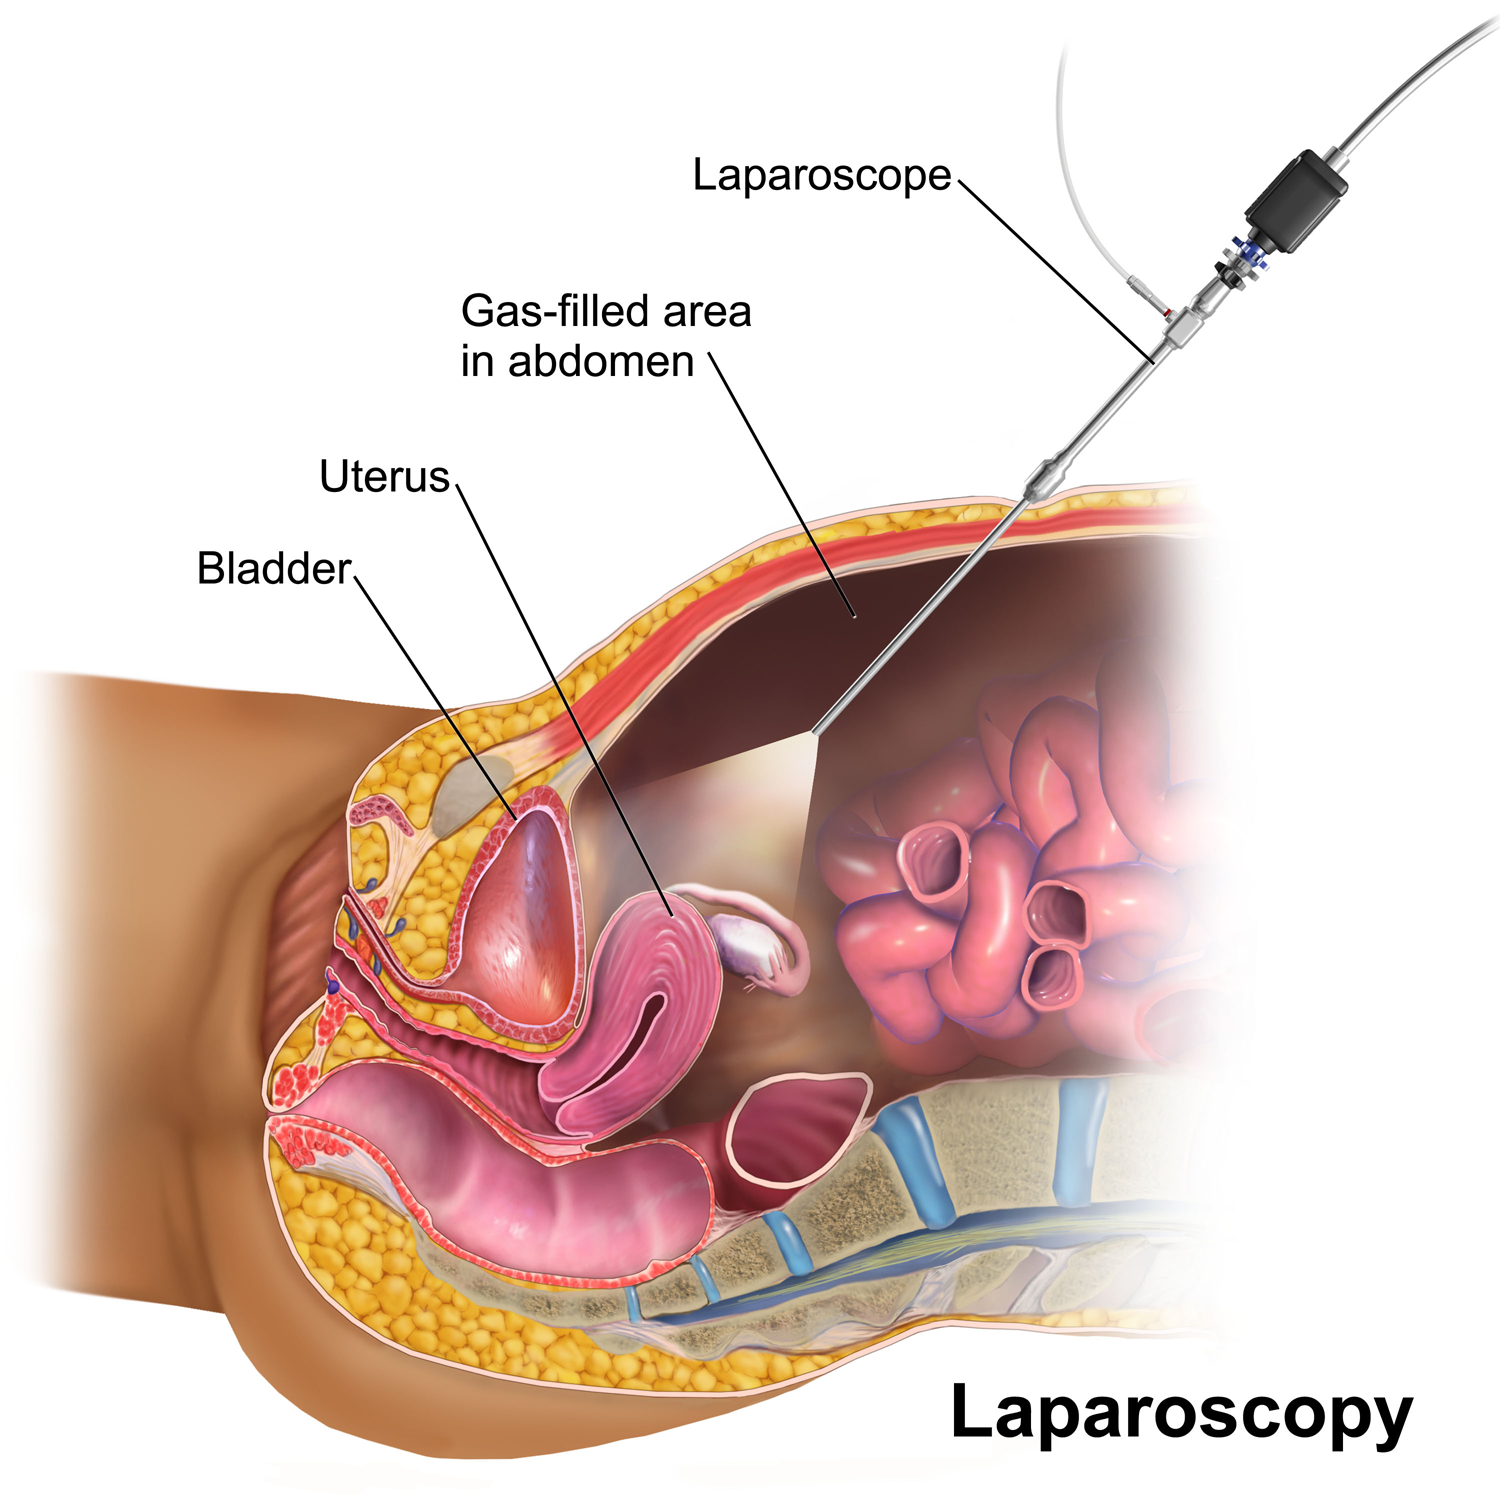
\includegraphics[width=0.4\linewidth]{images/intro_laparoscopy.png}
  \caption{Лапароскопія.}
  \label{fig:intro_laparoscopy}
\end{figure}

Лапароскопічні операції (рис. \ref{fig:intro_laparoscopy}) є кроком вперед проте мають ряд недоліків
\begin{itemize}
  \item Збільшення ймовірності інфекції.
  \item Суттєві больові відчуття у пацієнта\textbackslashпацієнтки після операції.
  \item Довший період реабілітації від хірургічного втручанння.
  \item Великий шрам у місці розтину.
\end{itemize}

Малоінвазивна робото хірургія. 


Більшість елементів сучасного приводу, конструкцій чи побутові речі виготовлені із гетерогенного матеріалу, зокрема із композиційного матеріалу або композиту. Тому виникає потреба у розробці методів, які б дозволяли розраховувати напружено-деформований стан, а також температуру.

Широко вживаними протягом кількох десятиріч методом розв'язування задач такого класу є проекційно-сітковий метод або метод скінчених елементів (МСЕ). Завдяки таким властивостям як розрідженість і симетричність матриць для класу задач у локально-неоднорідних тілах, різні варіанти МСЕ набули популярності.

Із МСЕ цілком успішно може конкурувати, а іноді бути ефективнішим,
велике сімейство методів граничних елементів
(МГЕ) \cite{benerdge-et-al} {[}4{]}{[}6{]}{[}7{]}{[}9{]}{[}12{]}{[}16{]}, які базуються
на ідеях розроблених С.Г.Міхліном{[}19{]}, Н.І.Мусхелішвілі{[}20{]},
В.Д.Купрадзе{[}17{]} та інші. Ці обставині особливо сприяють такі
переваги, як зменшення на одиницю геометричної розмірності задачі,
простота розв'язування для безмежних областей, можливість обчислювати у
лінійних задачах значення шуканих величин у довільній точці без нової
апроксимації, простота дискретизації.

У свою чергу серед класу МГЕ можна виділити такі методи як комплексний
метод граничних елементів (КМГЕ) і метод при граничних елементів (МПГЕ).
На відміну від КМГЕ, який є видозміненим варіантом класичного МГЕ, МПГЕ
базується на більш радикальніших ідеях. У порівнянні із МГЕ, МПГЕ
простіший для реалізації, проте у більшості випадків дає точніші
результати при тих самих затратах обчислювальних ресурсів.

Наукове завдання дисертаційної роботи -- розробка ефективного методу для
розв'язування задач термопружності у композитах є актуальною проблемою.

\textbf{Зв'язок роботи з науковими програмами, планами та
темами.} Робота виконувалась на кафедрі програмування львівського
національного університету імені Івана Франка, а також у інституті
прикладних проблем механіки і математики імені Ярослава Підстригача НАН
України, відділ термомеханіки в рамках держбюджетної теми ``Розробка
аналітико-чисельних методів дослідження напруженого стану неоднорідних
тіл з тепловими та залишковими деформаціями і дефектами структури''.
(!!! Номер теми !!!)

\textbf{Мета роботи та задачі дослідження.} Метою роботи є:

\begin{itemize}
\item
  побудова нових методів розв'язування задач термопружності у композитах
\item
  дослідження ефективності нових методів
\item
  порівняння швидкості збіжності і використання ресурсів із відомими
  методами
\end{itemize}

\emph{Об'єктом} дослідження є композити.

\emph{Предметом} дослідження є нові методи розв'язування задач
термопружності для композитів.

\emph{Методи дослідження.} Для розв'язування поставлених задач
використовується метод поєднання граничних і скінчених елементів.

\textbf{Наукова новизна одержаних результатів.} Наступні
результати отримані у роботі є новими:

\begin{enumerate}
\def\labelenumi{\arabic{enumi}.}
\item
  побудований метод на основі КМГЕ і МСЕ для розв'язування задачі
  теплопровідності у тілах із локальними неоднорідностями
\item
  для тіл із локальними неоднорідностями побудований метод на основі
  МПГЕ і МСЕ для розв'язування задач:

  \begin{enumerate}
  \def\labelenumii{\alph{enumii}.}
  \item
    пружності
  \item
    термопружності
  \end{enumerate}
\end{enumerate}

\textbf{Практичне значення отриманих результаті.} Отримані
результати дозволяють ефективніше розв'язувати актуальні проблеми, які
ставить перед нами народне господарство.

\textbf{Апробація результатів дисертації.} Основні результати
виконаних досліджень доповідалися та обговорювалися на:

\begin{enumerate}
\def\labelenumi{\arabic{enumi}.}
\item
  Восьмій Всеукраїнській науковій конференції (25-27 вересня 2001 р., м.
  Львів) ``Сучасні проблеми прикладної математики та інформатики'';
\item
  Дев'ятій Всеукраїнській науковій конференції (24-26 вересня 2002 р.,
  м. Львів) ``Сучасні проблеми прикладної математики та інформатики'';
\item
  Десятій Всеукраїнській науковій конференції (23-25 вересня 2003 р., м.
  Львів) ``Сучасні проблеми прикладної математики та інформатики'';
\item
  Одинадцятій Всеукраїнській науковій конференції (!!! 2004р., м. Львів)
  ``Сучасні проблеми прикладної математики та інформатики'';
\item
  Дванадцятій Всеукраїнській науковій конференції (4-6 жовтня 2005р., м.
  Львів) ``Сучасні проблеми прикладної математики та інформатики'';
\item
  Науковому семінарі ІППММ НАНУ імені Я.С.Підстригача, присвяченої
  пам'яті Є.Г.Грицька (22 квітня 2003 р., м. Львів);
\item
  Шостій Міжнародній науковій конференції (26-29 травня 2003 р., м.
  Львів) ``Математичні проблеми механіки неоднорідних структур'';
\item
  Семінар інституту прикладних проблем механіки та математики ім. Я.
  Підстригача
\end{enumerate}

У повному обсязі робота доповідалася на семінарі кафедри програмування
львівського національного університету імені Івана Франка.

\textbf{Публікації.} Результати досліджень висвітлені в 4 статтях
у журналах з переліку фахових видань ВАК України, в тому числі у
доповідях НАН України.

\textbf{Особистий внесок здобувача.} Всі результати дисертаційної
роботи отримано здобувачем самостійно.

\textbf{Структура та обсяг роботи.} Дисертація складається із
вступу і шести розділів основної частини, висновків, списку використаної
літератури із 37 найменувань.

У першому розділі описано підходи до розв'язування задач термопружності
і підхід, який був вибраний у даній роботи. Проаналізовано переваги і
недоліки кожного із запропонованих методів.

Другий розділ містить опис двох підходів для розв'язування задачі
теплопровідності. Перший підхід базується на ідеї предиктор-коректор, а
другий -- на рівняннях нев'язки у точках областей локальної
неоднорідності коефіцієнта теплопровідності.

Метод адитивного розчеплення оператора застосований для задачі пружності
для локально-неоднорідного тіла запропонований у третьому розділі. Даний
підхід був апробований для двох методів МГЕ і МПГЕ. Наведено порівняння
чисельних результатів для цих двох методів, а також порівняння методів
по інших критеріях, таких як простота реалізації, точність, діагональне
переважання матриць.

Четвертий розділ містить порівняльний аналіз МГЕ і МПГЕ при розв'язуванні задачі пружності у кусково-однорідному тілі. Наводяться рекомендації щодо застосування даних підходів для розв'язування задач такого класу.

У п'ятому розділі наведено підхід на основі МГЕ і МПГЕ для розв'язування
задачі термопружності у тілі із локально-неоднорідними властивостями
фізичних параметрів.

Програмне середовище Aspirant's Calculations Envinronment (ACE) було
створене для простого і зручного програмування запропонованих методів.
Структура даного середовища описана у шостому розділі. Також дано
рекомендації відносно використання даного середовища для програмування
подібних методів, яке вимагає невеликих зусиль спрямованих тільки на
побудову алгоритму, але не на організацію взаємодії між об'єктами.

\textbf{Усталені домовленості.} У цій праці кома перед індексом
означає похідну по змінній, яка відповідає цьому індексу, тобто
 ${f_{,j} = \partial}{f/\partial}x_{j}$, ${{f_{,ij} = \partial^{2}}{f/\partial}x_{i}\partial x_{j}}{}$,
при цьому викори­стовується німе сумування за індек­сами, які
повторюються.


\mainmatter %% turns on page numeration for pages below

\chapter{ЗАДАЧА ТЕПЛОПРОВІДНІСТЬ У М'ЯКИХ ТКАНИНАХ ТІЛА ЛЮДИНИ}

%Hidden cite for correct bibliography ordering
\nocite{bahvalov-et-al,tumor-thermal-modell,lung-tumor-thermal-conductivity,database-tissue-properties} 

\section{Огляд проблеми}

Використання новітніх підходів для виявлення аномалій в тілі людини, а також для виявлення ушкоджень після 
електро-коагуляції.

Тепловий ендоскоп як описано тут

Thermal endoscope based on cost-effective LWIR camera cores
Dumitru Scutelnic a, Giacomo Marchioro a, Salvatore Siracusano b, Paolo Fiorini a,
Riccardo Muradore a, Claudia Daffara a,

Також роблять для Da Vinci такі ендоскопи.

Потенційно новий прилад користь якого можна апробувати у симуляції.

Для цього треба створити модель м'яких тканин людини із ураженими клітинами. 

Симуляції уражених (ракових) клітин під час малоінвазиdної хіругії.

Рак легенів (\cite{lung-cancer}).

Традиційно за модель біотеплового обміну у тілі людини беруть рівняння Пеннеса.

pennes-1998-analysis-of-tissue-and-arterial-blood-temperatures-in-the-resting-human-forearm

Воно було сформульовано автором у його відомій статті у 1948 році і відтоді використовується для таких розрахуків.

% Для валідації моделі сформулюєм

\section{Формулюваня плоскої задачі}

Спочатку розв'яжемо плоский випадок із стаціонарним розподілом температури.
Візьмемо перетин області проведеннея малоінвазивного втручання

На (рис. \ref{fig:thermo_2d_domain}) зображено область перерізу, яка складається із трьох областей $\Omega_1$, 
$\Omega_2$ і $\Omega_3$. Зовнішня границя $\Gamma$ складається із двох частин $\Gamma_1$ і $\Gamma_2$, тобто 
$\Gamma=\Gamma_1\cap\Gamma_2$. 

\begin{figure}[ht!]
    \centering
    \begin{tikzpicture}
        \draw (1,3) rectangle (11,7);
        \draw (1,1) rectangle (11,3);
        \draw (6,2.5) circle (0.5);

        \draw[thick,->] (0,0) -- (12,0) node[anchor=north west] {x};
        \draw[thick,->] (0,0) -- (0,9) node[anchor=south east] {y};        
    
        \foreach \x in {0,...,4}
            \pgfmathtruncatemacro{\label}{\x * 10}
            \draw ( \x * 2.5 cm,1pt) -- ( \x * 2.5 cm,-1pt) node[anchor=north] {\label};
        \foreach \y in {0,...,3}
            \pgfmathtruncatemacro{\label}{\y * 10}
            \draw (1pt,\y * 2.5 cm) -- (-1pt,\y * 2.5 cm) node[anchor=east] {\label};
        
        \node at (11.5,2) {a};
        \node at (11.5,5) {b};
        \node at (6,7.5) {c};

        \node at (8,2) {$\Omega_1$};
        \node at (8,5) {$\Omega_2$};
        \node at (6,2.5) {$\Omega_3$};
        \node at (6,0.5) {$\Gamma_1$};

    \end{tikzpicture}
    
    \caption{Переріз тканин}
    \label{fig:thermo_2d_domain}
\end{figure}

Задача формулюється так:

\begin{equation}
    \label{eqn:thermo_2d_eqn}
    \nabla \cdot (k \nabla u) + \omega \rho_b C_b (T_c - u) + q_m  = 0
\end{equation}

На частині границі $\Gamma_2$ задані умови Діріхле, а на $\Gamma_1$ - Неймана.

\begin{equation}
    \label{eqn:thermo_2d_cond_1}
    u(z) = 36, z \in \Gamma_2
\end{equation}

\begin{equation}
    \label{eqn:thermo_2d_cond_2}
    \dfrac{\partial{u(z)}}{\partial{n}} = 0, z \in \Gamma_1
\end{equation}

\noindentУ рівнянні \ref{eqn:thermo_2d_eqn} використовуються наступні позначення:

\begin{center}
    \begin{tabular}{|c|c|} 
        \hline
            k & коефіцієнт тепловідності \\
        \hline
            \(\omega\) & перфузія крові через орган \\
        \hline
            \(\rho_b\) & густина крові \\
        \hline
            \(C_b\) & питома теплоємність крові \\
        \hline
            \(T_c\) & внутрішня температура тіла \\
        \hline
            \(q_m\) & метаболічне тепло у тканині \\
        \hline
    \end{tabular}
\end{center}

Головним джерелом даних для фізичних параметрів органів тіла була онлайн база даних \cite{database-tissue-properties}.

\textbf{Коефіцієнт тепропровідності} Коефіцієнт тепропровідності у ракових утвореннях взято із статті 
\cite{lung-tumor-thermal-conductivity}. Модель злоякісного утворення взята із статті \cite{tumor-thermal-model}.
Коефіцієнт тепловідності у пухлині рівний 0.495 Вт/мК, у прилеглих тканинах 0.445 Вт/мК і у здорових тканинах 
0.19 Вт/мК. Злоякісна пухлини предаставлена областю $\Omega_3$. Відповідно коефіцієнт теплопровідності k буде залежати
від координат і його можна представити у вигляді наступої функції:

\begin{equation}
    \label{eqn:thermo_2d_thermal_conductivity}
    k(x, y) = cos(\frac{\pi}{2}((x - x_3)^2 + (y - y_3)^2)) + 1.0
\end{equation}

\noindent де $\chi_3$ - характеристична функція області $\Omega_3$, a ($x_3$, $y_3$) - центр області.

\textbf{швидкість руху крові у тканинах} \textbf{blood perfusion} $$\omega$$ blood perfusion rate $$\omega$$ was found to be between 1.2 and 1.8 mL
blood/min/100 g tissue (from: HEAT TRANSFER APPLICATIONS IN BIOLOGICAL SYSTEMS)

In humans, there are several tissue regions, such as kidney, heart, and choriocapillaris in the eye, pos-
sessing a high blood perfusion rate. The measured blood perfusion rate in the kidney is approxi-
mately 500 mL/min/100 g tissue (Holmes, 1997). In the heart, the blood perfusion rate is around
300 mL/min/100 g which serves for the energy need of pumping the heart. The choriocapillaris in
the eyes is a meshed structure within two thin sheets. Its blood perfusion rate is very high and can
be as much as 8000 mL/min/100 g tissue (from: HEAT TRANSFER APPLICATIONS IN BIOLOGICAL SYSTEMS)

Звідси випливає, що коефіцієнт тепропровідності залежить від координат і може бути наближений кусково ламаною функцією 
або функціями вищого порядку, наприклад квадратичною. Для даного прикладу пропонується використати:

% \begin{equation}
%     \label{eqn:thermo_2d_thermal_conductivity}
%     (np.cos(0.5 * np.pi / radius * (np.power(x - 1.0, 2) + np.power(y - 1.0, 2))) + 1.0
% \end{equation}


Відповідно якщо задати 

\textbf{Густина} $$\rho_b$$ - густина крові 1050 кг/$$m^3$$ %(джерело: https://itis.swiss/virtual-population/tissue-properties/database/density/)

\textbf{Питома теплоємність крові?} $$C_b$$ = 3617 Дж/Kg/C %(джерело: https://itis.swiss/virtual-population/tissue-properties/database/heat-capacity/)

$$T_c$$ - базова температура тіла 37 Цельсія

$$q_m$$ 4.2 KK/Kg/◦ C та сама стаття  1.21

qm is the metabolic heat generation in the tissue

\begin{center}
    \begin{tabular}{|c|c|c|c|} 
     \hline
     Густина крові & \(\rho_b\) & \(\text{кг}/\text{м}^3\) \\ 
     \hline
     Питома теплоємність крові & 3617 & Дж/кг/С \\ 
     \hline
    \end{tabular}
\end{center}

сіффісфіівів

\section{Дискретизація рівнянь}

\section{Розв'язок}

\section{Формулюваня просторової задачі}

\section{Дискретизація рівнянь}

\section{Розв'язок}

\section{Висновок}


% \chapter{ЗАДАЧА ТЕПЛОПРОВІДНОСТІ ДЛЯ ПЛОСКОГО ТІЛА ІЗ ЛОКАЛЬНО-НЕОДНОРІДНИМ ВКЛЮЧЕННЯМ}

%Hidden cite for correct bibliography ordering
\nocite{bahvalov-et-al,benerdge-et-al} 

\section{Постановка задачі}

Нехай характеристика середовища $\Lambda (z)$ стосовно певного фізичного процесу,
модельованого потенціалом безвихрового векторного поля,
(теплопровідності, дифузії, електромагнітостатики, пружного руху
твердого тіла, течією ґрунтових вод тощо) є неперервною функцією
декартових координат $z = (x, y)$,
сталою скрізь у плоскій однозв'язній області $ \Omega $ з простим
замкнутим краєм $ \Gamma = {\Gamma_{1} \cup \Gamma_{2}} $, за
винятком скінченої сукупності локальних неоднорідних включень
$\Omega_{k}\subset\Omega$ ($\Omega_k \underset {k \neq l} \cap \Omega_l = \varnothing$, 
$\partial \Omega_k \cap \Gamma = \varnothing $, $ k,l = \overline{1,K} $).

Розглянемо змішану крайову задачу для основного рівняння стаціонарного
поля в локально-неоднорідному середовищі

\begin{equation}
\label{eqn:teploprovidnist_1}
div(\Lambda(z) \nabla \theta (z) ) = 0, z \in \Omega
\end{equation}

\begin{equation}
\label{eqn:teploprovidnist_2}
\theta(z) = p(z), z\in\Gamma_{1},
\Lambda(z) \frac{\partial \theta (z)}{\partial n}  = -q(z), z\in\Gamma_{2}
\end{equation}

де

\begin{equation}
\label{eqn:teploprovidnist_3}
\Lambda(z)=1+\sum_{k=1}^{K}a_k\lambda_k(z)\chi_k(z), z \in \Omega
\end{equation}
    
$a_k=const_k > -1$; $ \lambda_k(z) $ -- якісна характеристика провідності середовища в
$\Omega_{k} (k=\overline{1,K})$, причому $\lambda_{k}(z) \geq 0$, $\displaystyle \max_{\Omega_k} \lambda_k (z) = 1$, 
$\lambda_{k}(z)_{z\in\partial\Omega_{k}} = 0$; $\chi_{k}(z)$ -- характеристична функція області
$\Omega_{k}$.

Враховуючи (\ref{eqn:teploprovidnist_3}), задача (\ref{eqn:teploprovidnist_1})(\ref{eqn:teploprovidnist_2}) набуде вигляду:

\begin{equation}
\label{eqn:teploprovidnist_4}
\nabla^{2} \theta = -\sum_{k=1}^{K}a_k B_k[\theta]\chi_k \text{ в } \Omega
\end{equation}

\begin{equation}
\label{eqn:teploprovidnist_5}
\theta = p \text{ на } \Gamma_1; \frac{\partial\theta}{\partial \overrightarrow{n}} = -q \text{ на } \Gamma_2,
\end{equation}

де $B_k[\bullet]=\frac{\nabla\lambda_k\nabla[\bullet]}{1+a_k\lambda_k}$, $\nabla$ - оператор Гамільтона.

\section{Метод предиктор-коректор}

\subsection{Суть методу}

Розглянемо послідовність плоских змішаних крайових задач для основного
рівняння стаціонарного поля

\begin{equation}
\label{eqn:teploprovidnist_6}
div \Lambda_{n}(z) \nabla \phi_{n}(z) = 0, z\in\Omega
\end{equation}

\begin{equation}
\label{eqn:teploprovidnist_7}
\phi_{n}{(z) = \phi_{s}}(z), z\in\Gamma_{1}
\end{equation}

\begin{equation}
\label{eqn:teploprovidnist_8}
{\frac{\partial\phi_{n}(z)}{\partial\overrightarrow{n}} = {- \psi_{s}}}(z), z\in\Gamma_{2}
\end{equation}
    
за умови, що характеристика середовища
$\Lambda_{n}(z)({n = \overline{0,N}})$ (коефіцієнт
теплопровідності, коефіцієнт дифузії тощо) для кожної з цих задач є
неперервною функцією декартових координат
$z = ( {x,y} )$, сталою скрізь в однозв'язній області
$\Omega$ з простим замкнутим краєм
$\Gamma = {\Gamma_{1} \cup \Gamma_{2}}$, за винятком скінченої
сукупності неоднорідних включень $\Omega_{k}\subset\Omega$
($\Omega_{k}\underset{k \neq l} \cap {\Omega_{l} = \varnothing}$,
$\partial\Omega_{k} \cap {\Gamma =}$,
$k,{l = \overline{1,K}}$), геометрія та конфігурація розташування
яких фіксовані для всіх $n$ одночасно. А саме:

\begin{equation}
\label{eqn:teploprovidnist_9}
\Lambda_{n}{(z) = {1 + {\sum\limits_{k = 1}^{K}{a_{\mathit{\text{nk}}}\lambda_{k}(z)\chi_{k}(z)}}}}, z\in\Omega
\end{equation}
    
де $\lambda_{k}(z)$ -- якісна характеристика
провідності середовища в області $\Omega_k$ ($k = \overline{1,K}$), причому
$\lambda_{k}{(z) \geq 0}$, $\underset{\Omega_{k}}{\text{max}}\lambda_{k}(z){= 1}$,
$\lambda_{k}(z)_{z\in\partial\Omega_{k}} = 0$; $\chi_{k}(z)$ -- характеристична функція області
$\Omega_k$; $\{ a_{nk}\}$ -- монотонна послідовність ($n = \overline{0,N}$) для кожного
конкретного $k$, така, що $a_{0k} = 0$,
$a_{\mathit{\text{nk}}} > {- 1}$.

% Застосуємо до оператора основного рівняння стаціонарного поля (2.6),
% враховуючи (2.9), операції методу адитивного розщеплення операторів.
% Внаслідок цього (2.6) набуде вигляду

% $\nabla^{2}{\phi_{n} = P_{n}}\left\lbrack \phi_{n} \right\rbrack$
% в \[\Omega{}\],(2.10)

% де
% ${\nabla = \frac{\partial}{\partial x}}{\overrightarrow{i} + \frac{\partial}{\partial y}}\overrightarrow{j}$
% -- оператор Гамільтона;
% $P_{n}{\left\lbrack {} \right\rbrack = {- \Lambda_{n}^{- 1}}}{\sum\limits_{k = 1}^{K}{a_{\mathit{\text{nk}}}\nabla\lambda_{k}\nabla\left\lbrack {} \right\rbrack}}\chi_{k}$
% -- оператор, який враховує додатковий вплив неоднорідностей.

% Отже, маємо послідовність змішаних задач (2.10), (2.7), (2.8) для
% визначення розв'язків $\phi_{n}(z)$
% ($n = \overline{0,N}$).

% \hypertarget{ux43fux43eux431ux443ux434ux43eux432ux430-ux43fux440ux43eux446ux435ux434ux443ux440ux438-ux442ux438ux43fux443-ux43fux440ux43eux433ux43dux43eux437ux43aux43eux440ux435ux43aux442ux443ux432ux430ux43dux43dux44f}{%
% \subsubsection[2.2.2. Побудова процедури типу
% прогноз--коректування]{\texorpdfstring{\protect\hypertarget{anchor-32}{}{}\protect\hypertarget{anchor-33}{}{}2.2.2.
% Побудова процедури типу
% прогноз--коректування}{2.2.2. Побудова процедури типу прогноз--коректування}}\label{ux43fux43eux431ux443ux434ux43eux432ux430-ux43fux440ux43eux446ux435ux434ux443ux440ux438-ux442ux438ux43fux443-ux43fux440ux43eux433ux43dux43eux437ux43aux43eux440ux435ux43aux442ux443ux432ux430ux43dux43dux44f}}

% Для вибраної конкретної\textbf{ }геометрії неоднорідних включень та
% конкретної конфігурації їхнього розташування в \[\Omega{}\] побудуємо
% єдину процедуру, яка дає змогу розв'язувати відразу цілу низку задач
% типу (2.10), (2.7), (2.8), що відрізняються характеристиками середовища
% \[\Lambda_{n$($n = \overline{0,N}$). У цьому разі внаслідок
% послідовного застосування аналогічно до прийому попереднього моделювання
% шуканого розв'язку у правій частині (2.10) перейдемо до задач відносно
% ${\phi_{n}^{} = \phi_{n}^{}}(z)$.

% Ітерації пропонованої процедури для визначення послідовності функцій
% \[\phi_{i}^{$задамо такими формулами:

% $\nabla^{2}{\phi_{i}^{{}^{m}} = P_{i}}\left\lbrack {\hat{\phi}}_{i^{m - 1}} \right\rbrack$
% в \[\Omega{}\];(2.11)

% $\phi_{i}^{{}^{m}} = \phi_{s}$ на \[\Gamma_{1$;(2.12)

% $\frac{\partial\phi_{i}^{{}^{m}}}{\partial\overrightarrow{n}} = {- \psi_{s}}$
% на \[\Gamma_{2$;(2.13)

% $i = \overline{0,N}$; $m = \overline{1,M_{i}}$,

% де $\hat{\phi}}_{i}^{m - 1$-- апроксимація чергової ітерації
% розв'язку \[\phi_{i}^{{}^{m - 1}$задачі при характеристиці
% середовища \[\Lambda_{i$, причому
% ${\hat{\phi}}_{i + 1}^{0} = {\hat{\phi}}_{i}^{M_{i}}$;
% \[\]$\hat{\phi}}_{i}^{M_{i}$-- апроксимація \emph{відкоректованого
% }\[M_{i$ ітераціями розв'язку задачі при характеристиці середовища
% \[\Lambda_{i$; $\hat{\phi}}_{i + 1}^{0$ -- апроксимація
% початкового наближення \emph{прогнозованого }розв'язку при
% \[\Lambda_{i + 1$; $\hat{\phi}}_{0}^{0$ -- апроксимація
% розв'язку наступної задачі для однорідної області

% $\nabla^{2}{\phi_{0} = 0}$ в \[\Omega{}\];

% $\phi_{0} = \phi_{s}$ на \[\Gamma_{1$;
% $\frac{\partial\phi_{0}}{\partial\overrightarrow{n}} = {- \psi_{s}}$
% на \[\Gamma_{2$;

% Розв'язок кожної із задач (2.11) -- (2.13) зобразимо у вигляді

% $\phi_{i}^{{}^{m}}{(z) = \varphi_{i}^{m}}{(z) - \Phi_{i}^{m}}(z)$,

% де

% $\Phi_{i}^{m}{(z) = \frac{1}{2\pi}}{\sum\limits_{k = 1}^{K}{a_{\mathit{\text{ik}}}{\int\limits_{\Omega_{k}}{\text{ln}( {( {x - x^{}} )^{2} + ( {y - y^{}} )^{2}} )}}}^{\frac{- 1}{2}}}{\Lambda_{i}^{- 1}( z^{} )}{\nabla\lambda_{k}( z^{} )}{\nabla{\hat{\phi}}_{i}^{m - 1}( z^{} )}{d\Omega_{k}( z^{} )}$--
% частковий розв'язок рівняння (2.11);
% $\varphi_{i}^{m}(z)$ -- розв'язок наступної змішаної
% задачі для рівняння Лапласа

% $\nabla^{2}{\varphi_{i}^{m} = 0}$ в \[\Omega{}\];

% $\varphi_{i}^{m} = {\phi_{s} + \Phi_{i}^{m}}$ на \[\Gamma_{1$;
% $\frac{\partial\psi_{i}^{m}}{\partial\overrightarrow{s}} = {{- \psi_{s}} + \frac{\partial\Phi_{i}^{m}}{\partial\overrightarrow{n}}}$
% на \[\Gamma_{2$,

% який легко можна знайти, використовуючи інтегральну формулу Коші для
% функції
% $\omega_{i}^{m}{(z) = \varphi_{i}^{m}}{(z) + {i \cdot \psi_{i}^{m}}}(z)$
% комплексної змінної \[z{}\]( $\varphi_{i}^{m}(z)$ --
% потенціал; $\psi_{i}^{m}(z)$ -- функція потоку;
% \[\overrightarrow{s$ -- одиничний вектор, дотичний до
% \[\Gamma_{2$ ) згідно з прямим чи непрямим формулюванням алгоритму
% КМГЕ.

% \hypertarget{ux447ux438ux441ux43bux43eux432ux456-ux440ux435ux437ux443ux43bux44cux442ux430ux442ux438}{%
% \subsubsection[2.2.3. Числові
% результати]{\texorpdfstring{\protect\hypertarget{anchor-34}{}{}2.2.3.
% Числові
% результати}{2.2.3. Числові результати}}\label{ux447ux438ux441ux43bux43eux432ux456-ux440ux435ux437ux443ux43bux44cux442ux430ux442ux438}}

% Об'єктом числових досліджень було вибрано послідовність змішаних
% крайових задач теплопровідності типу (2.6) -- (2.9) в області
% $\Omega = {( {x^{-};x^{+}} ) \times ( {y^{-};y^{+}} )}$
% з краєм
% \includegraphics[width=0.7646in,height=0.2217in]{./ObjectReplacements/Obj217},
% де\[\]\textbf{; }\[\]\textbf{;}

% \[\]\textbf{; }\[\]\textbf{ , }яка містить область локальної
% неоднорідності \[\].

% Граничні умови, схарактеризовані так: \[\]\textbf{; }\[\]\textbf{.}

% Якісну характеристику теплопровідності середовища було задано у вигляді

% \[\]\textbf{;
% }\includegraphics[width=0.5429in,height=0.2217in]{./ObjectReplacements/Obj226}\textbf{.}

% Усі графіки, показані на рис. 2.1--2.3, стосуються таких конкретних
% значень параметрів: \[\]; \[\]; \[\]; \[\]; \[\]

% \includegraphics[width=5.111in,height=3.528in]{Pictures/100000000000020200000163358C6F063C52CE42.png}\includegraphics[width=5.111in,height=3.25in]{Pictures/10000000000001EB0000013832389E2C121C29E6.png}

% Рис. 2.1

% На рис. 2.1 наочно простежується залежність температурного поля (рис.
% 2.1,а) від властивостей середовища (рис. 2.1,б). Видно, що зі
% збільшенням відстані до області локальної неоднорідності
% (\includegraphics[width=0.5283in,height=0.2217in]{./ObjectReplacements/Obj232})
% зменшується її вплив на температурне поле, тобто розв'язок задачі щораз
% менше відрізняється від розв'язку аналогічної задачі для випадку
% однорідного середовища.

% \includegraphics[width=5.111in,height=2.889in]{Pictures/100000000000031C000001C112ECC8EDD043C886.png}

% Рис. 2.2

% \includegraphics[width=5.111in,height=2.889in]{Pictures/100000000000031C000001C1A825D2F7BF570EC8.png}

% Рис. 2.3

% Зображені на рис. 2.2, рис. 2.3 графіки демонструють зміну розв'язків
% крайових задач (2.6)--(2.9) уздовж осі
% \includegraphics[width=0.4in,height=0.2217in]{./ObjectReplacements/Obj233},
% що проходить через центр області локальної неоднорідності, де
% найяскравіше виявляються закономірності впливу теплофізичних
% властивостей середовища на розв'язок.

% Крива 1 на рис. 2.2 -- розв'язок задачі без неоднорідності; криві 2--5
% -- розв'язки задач за наявної неоднорідності радіуса
% \includegraphics[width=0.5283in,height=0.2217in]{./ObjectReplacements/Obj234}
% і максимальних відхиленнях у ній значень коефіцієнта теплопровідності
% від значення у решті області, відповідно, у 3, 5, 7, 9 разів. Криві 1--5
% добре демонструють збіжність послідовності розв'язків крайових задач
% (2.6)--(2.9)
% (\includegraphics[width=0.4854in,height=0.2354in]{./ObjectReplacements/Obj235}),
% а також щоразу яскравіший прояв із зростанням провідності ефекту
% ``плато''.

% Графіки на рис. 2.3 одержані при
% \includegraphics[width=0.3646in,height=0.1783in]{./ObjectReplacements/Obj236}
% і значеннях
% \includegraphics[width=1.0429in,height=0.2217in]{./ObjectReplacements/Obj237}
% (відповідно, криві 2--4). Крива 1 відповідає розв'язку задачі для
% однорідного середовища. Можемо спостерігати розширення сфери впливу
% неоднорідності на розв'язок із збільшенням розмірів неоднорідності.

% \hypertarget{ux43cux435ux442ux43eux434-ux43fux43eux454ux434ux43dux430ux43dux43dux44f-ux433ux440ux430ux43dux438ux447ux43dux438ux445-ux435ux43bux435ux43cux435ux43dux442ux456ux432-ux456ux437-ux441ux43aux456ux43dux447ux435ux43dux438ux43cux438-ux435ux43bux435ux43cux435ux43dux442ux430ux43cux438}{%
% \subsection[2.3. Метод поєднання граничних елементів із скінченими
% елементами]{\texorpdfstring{\protect\hypertarget{anchor-35}{}{}2.3.
% Метод поєднання граничних елементів із скінченими
% елементами}{2.3. Метод поєднання граничних елементів із скінченими елементами}}\label{ux43cux435ux442ux43eux434-ux43fux43eux454ux434ux43dux430ux43dux43dux44f-ux433ux440ux430ux43dux438ux447ux43dux438ux445-ux435ux43bux435ux43cux435ux43dux442ux456ux432-ux456ux437-ux441ux43aux456ux43dux447ux435ux43dux438ux43cux438-ux435ux43bux435ux43cux435ux43dux442ux430ux43cux438}}

% \hypertarget{ux441ux443ux442ux44c-ux43cux435ux442ux43eux434ux443-1}{%
% \subsubsection[2.3.1. Суть
% методу]{\texorpdfstring{\protect\hypertarget{anchor-36}{}{}2.3.1. Суть
% методу}{2.3.1. Суть методу}}\label{ux441ux443ux442ux44c-ux43cux435ux442ux43eux434ux443-1}}

% Припустимо, що нам відома апроксимація
% \includegraphics[width=0.1283in,height=0.2071in]{./ObjectReplacements/Obj238}
% функції розв'язку
% \includegraphics[width=0.1283in,height=0.1646in]{./ObjectReplacements/Obj239}
% задачі (2.4),(2.5) в області кожної з локальних неоднорідностей
% \includegraphics[width=0.2071in,height=0.2071in]{./ObjectReplacements/Obj240}.
% Використаємо
% \includegraphics[width=0.1283in,height=0.2071in]{./ObjectReplacements/Obj241}
% у правій частині (2.4). Потрактуємо розв'язок
% \includegraphics[width=0.1354in,height=0.1646in]{./ObjectReplacements/Obj242}
% одержаної крайової задачі

% \includegraphics[width=1.2929in,height=0.4in]{./ObjectReplacements/Obj243}
% в
% \includegraphics[width=0.1646in,height=0.15in]{./ObjectReplacements/Obj244};(2.14)

% \includegraphics[width=0.3783in,height=0.1929in]{./ObjectReplacements/Obj245}
% на
% \includegraphics[width=0.1646in,height=0.2071in]{./ObjectReplacements/Obj246};
% \includegraphics[width=0.5429in,height=0.3854in]{./ObjectReplacements/Obj247}
% на
% \includegraphics[width=0.1783in,height=0.2071in]{./ObjectReplacements/Obj248},(2.15)

% як аналог розв'язку вихідної задачі.

% Далі розв'язок задачі (2.14),(2.15) зобразимо у вигляді

% \includegraphics[width=1.5in,height=0.4in]{./ObjectReplacements/Obj249},(2.16)

% де

% \includegraphics[width=2.1783in,height=0.4429in]{./ObjectReplacements/Obj250},(2.17)

% а
% \includegraphics[width=0.3217in,height=0.2354in]{./ObjectReplacements/Obj251}
% - розв'язок задачі для рівняння Лапласа з видозміненими крайовими
% умовами

% \includegraphics[width=0.4854in,height=0.1929in]{./ObjectReplacements/Obj252}
% в
% \includegraphics[width=0.1646in,height=0.15in]{./ObjectReplacements/Obj253};(2.18)

% \includegraphics[width=1.1146in,height=0.35in]{./ObjectReplacements/Obj254}
% на
% \includegraphics[width=0.1646in,height=0.2071in]{./ObjectReplacements/Obj255};
% \includegraphics[width=1.2929in,height=0.4in]{./ObjectReplacements/Obj256}
% на
% \includegraphics[width=0.1783in,height=0.2071in]{./ObjectReplacements/Obj257},(2.19)

% де
% \includegraphics[width=1.4146in,height=0.4283in]{./ObjectReplacements/Obj258}.

% Шуканий розв'язок задачі (2.18), (2.19) проінтерпретуємо наступним чином
% \includegraphics[width=0.5429in,height=0.1646in]{./ObjectReplacements/Obj259},
% де
% \includegraphics[width=1.4in,height=0.2354in]{./ObjectReplacements/Obj260}
% - аналітична в
% \includegraphics[width=0.3783in,height=0.1929in]{./ObjectReplacements/Obj261}
% функція комплексної змінної
% \includegraphics[width=0.5717in,height=0.1929in]{./ObjectReplacements/Obj262},
% причому потенціал
% \includegraphics[width=0.1283in,height=0.1354in]{./ObjectReplacements/Obj263}
% та функція потоку
% \includegraphics[width=0.1146in,height=0.1354in]{./ObjectReplacements/Obj264}
% є гармонійними в
% \includegraphics[width=0.3783in,height=0.1929in]{./ObjectReplacements/Obj265}.

% Беручи до уваги, що
% \includegraphics[width=0.5146in,height=0.3854in]{./ObjectReplacements/Obj266},
% де
% \includegraphics[width=0.1283in,height=0.1783in]{./ObjectReplacements/Obj267}
% - одиничний додатньоорієнтований (проти руху стрілок годинника) вектор,
% дотичний до
% \includegraphics[width=0.1354in,height=0.15in]{./ObjectReplacements/Obj268},
% перейдемо до розв'язування такої крайової задачі:

% \includegraphics[width=0.6783in,height=0.2354in]{./ObjectReplacements/Obj269}
% в
% \includegraphics[width=0.1646in,height=0.15in]{./ObjectReplacements/Obj270},(2.20)

% \includegraphics[width=1.5in,height=0.35in]{./ObjectReplacements/Obj271}
% на
% \includegraphics[width=0.1646in,height=0.2071in]{./ObjectReplacements/Obj272};(2.21)

% \includegraphics[width=1.6646in,height=0.4429in]{./ObjectReplacements/Obj273}
% на
% \includegraphics[width=0.1783in,height=0.2071in]{./ObjectReplacements/Obj274}.(2.22)

% Для довільної точки
% \includegraphics[width=0.1283in,height=0.1283in]{./ObjectReplacements/Obj275}
% заданої однозв'язної області
% \includegraphics[width=0.1646in,height=0.15in]{./ObjectReplacements/Obj276}
% з простим замкнутим додатньоорієнтованим краєм
% \includegraphics[width=0.1354in,height=0.15in]{./ObjectReplacements/Obj277}
% справедлива інтегральна формула Коші

% \includegraphics[width=1.3783in,height=0.4283in]{./ObjectReplacements/Obj278},(2.23)

% яка слугуватиме основою наступних викладок.

% \hypertarget{ux434ux438ux441ux43aux440ux435ux442ux438ux437ux430ux446ux456ux44f-ux433ux435ux43eux43cux435ux442ux440ux456ux457-ux442ux430-ux432ux438ux437ux43dux430ux447ux435ux43dux43dux44f-ux430ux43fux440ux43eux43aux441ux438ux43cux430ux446ux456ux439}{%
% \subsubsection[2.3.2. Дискретизація геометрії та визначення
% апроксимацій]{\texorpdfstring{\protect\hypertarget{anchor-37}{}{}\protect\hypertarget{anchor-38}{}{}2.3.2.
% Дискретизація геометрії та визначення
% апроксимацій}{2.3.2. Дискретизація геометрії та визначення апроксимацій}}\label{ux434ux438ux441ux43aux440ux435ux442ux438ux437ux430ux446ux456ux44f-ux433ux435ux43eux43cux435ux442ux440ux456ux457-ux442ux430-ux432ux438ux437ux43dux430ux447ux435ux43dux43dux44f-ux430ux43fux440ux43eux43aux441ux438ux43cux430ux446ux456ux439}}

% Дискретизуємо
% \includegraphics[width=0.1354in,height=0.15in]{./ObjectReplacements/Obj279}послідовністю
% \includegraphics[width=0.1646in,height=0.1646in]{./ObjectReplacements/Obj280}
% граничних елементів
% \includegraphics[width=0.1783in,height=0.2071in]{./ObjectReplacements/Obj281}
% (таких, що
% \includegraphics[width=0.35in,height=0.4in]{./ObjectReplacements/Obj282}
% апроксимує
% \includegraphics[width=0.1646in,height=0.2071in]{./ObjectReplacements/Obj283},
% а
% \includegraphics[width=0.4283in,height=0.4in]{./ObjectReplacements/Obj284}
% -
% \includegraphics[width=0.1783in,height=0.2071in]{./ObjectReplacements/Obj285}),
% моделюючи геометрію кожного з елементів за допомогою вектора
% \includegraphics[width=0.1354in,height=0.2071in]{./ObjectReplacements/Obj286}
% базових інтерполюючих функцій, пов'язаних із локальною нормалізованою
% координатою
% \includegraphics[width=0.1283in,height=0.1646in]{./ObjectReplacements/Obj287}.
% Вздовж кожного з елементів апроксимуємо
% \includegraphics[width=0.15in,height=0.1354in]{./ObjectReplacements/Obj288}
% інтерполяційним поліномом

% \includegraphics[width=1.0571in,height=0.2354in]{./ObjectReplacements/Obj289},(2.24)

% де
% \includegraphics[width=0.1783in,height=0.2071in]{./ObjectReplacements/Obj290}
% - вектор невідомих вузлових значень
% функції\includegraphics[width=0.15in,height=0.1354in]{./ObjectReplacements/Obj291}.

% Кожну з областей
% \includegraphics[width=0.2071in,height=0.2071in]{./ObjectReplacements/Obj292}
% дискретизуємо системою ермітових чотирикутних елементів
% \includegraphics[width=0.2646in,height=0.2071in]{./ObjectReplacements/Obj293}\includegraphics[width=0.6929in,height=0.2929in]{./ObjectReplacements/Obj294}
% і представимо
% \includegraphics[width=0.1283in,height=0.2071in]{./ObjectReplacements/Obj295}
% пробною функцією {[}\protect\hyperlink{anchor-39}{24}{]}

% \includegraphics[width=1.4854in,height=0.25in]{./ObjectReplacements/Obj296},(2.25)

% де
% \includegraphics[width=0.2217in,height=0.2354in]{./ObjectReplacements/Obj297}
% - вектор невідомих вузлових значень функції
% \includegraphics[width=0.1283in,height=0.2071in]{./ObjectReplacements/Obj298},
% значень її перших та змішаних похідних на елементі
% \includegraphics[width=0.2646in,height=0.2071in]{./ObjectReplacements/Obj299},
% \includegraphics[width=0.15in,height=0.2071in]{./ObjectReplacements/Obj300}
% - вектор базових функцій у локальній системі координат
% \includegraphics[width=0.65in,height=0.2354in]{./ObjectReplacements/Obj301}.

% Враховуючи (2.24), дискретний аналог (2.23) набуде вигляду

% \includegraphics[width=1.7354in,height=0.4571in]{./ObjectReplacements/Obj302}.(2.26)

% Зважаючи на (2.25),
% \includegraphics[width=0.1646in,height=0.2071in]{./ObjectReplacements/Obj303}
% (подібно й
% \includegraphics[width=0.1929in,height=0.2071in]{./ObjectReplacements/Obj304})
% зобразимо

% \includegraphics[width=1.7783in,height=0.2929in]{./ObjectReplacements/Obj305},

% де

% \includegraphics[width=3.5283in,height=0.4717in]{./ObjectReplacements/Obj306}.

% \hypertarget{ux43fux43eux431ux443ux434ux43eux432ux430-ux441ux438ux441ux442ux435ux43cux438-ux440ux456ux432ux43dux44fux43dux44c-ux434ux43bux44f-ux437ux43dux430ux445ux43eux434ux436ux435ux43dux43dux44f-ux432ux443ux437ux43bux43eux432ux438ux445-ux437ux43dux430ux447ux435ux43dux44c}{%
% \subsubsection[2.3.3. Побудова системи рівнянь для знаходження вузлових
% значень]{\texorpdfstring{\protect\hypertarget{anchor-40}{}{}\protect\hypertarget{anchor-41}{}{}2.3.3.
% Побудова системи рівнянь для знаходження вузлових
% значень}{2.3.3. Побудова системи рівнянь для знаходження вузлових значень}}\label{ux43fux43eux431ux443ux434ux43eux432ux430-ux441ux438ux441ux442ux435ux43cux438-ux440ux456ux432ux43dux44fux43dux44c-ux434ux43bux44f-ux437ux43dux430ux445ux43eux434ux436ux435ux43dux43dux44f-ux432ux443ux437ux43bux43eux432ux438ux445-ux437ux43dux430ux447ux435ux43dux44c}}

% У підрозділі 2.2 запропонована процедура типу прогноз-коректування до
% розв'язування зразу цілої серії задач класу (2.1), (2.2) для конкретно
% вибраної кількості, геометрії та конфігурації розташування неоднорідних
% включень, але різних функцій, що описують провідність середовища. Зараз
% же представимо принципово інший підхід, а саме: систему рівнянь для
% визначення вузлових значень побудуємо за методом зважених нев'язок,
% уведених як для крайових умов, так і для областей локальних включень. У
% матричній формі система матиме, зокрема, якщо скористатися непрямим
% формулюванням методу граничних елементів, такий загальний вигляд:

% \includegraphics[width=2.3217in,height=1.1in]{./ObjectReplacements/Obj307}\includegraphics[width=0.3354in,height=1.5429in]{./ObjectReplacements/Obj308}=\includegraphics[width=0.2646in,height=1.0717in]{./ObjectReplacements/Obj309},(2.27)

% де
% \includegraphics[width=0.1283in,height=0.1783in]{./ObjectReplacements/Obj310},
% \includegraphics[width=0.15in,height=0.2354in]{./ObjectReplacements/Obj311},
% ...,
% \includegraphics[width=0.1783in,height=0.2354in]{./ObjectReplacements/Obj312},
% \includegraphics[width=0.1146in,height=0.1783in]{./ObjectReplacements/Obj313}
% - вектори невідомих вузлових значень відповідно потенціалу на
% дискретному аналозі
% \includegraphics[width=0.1783in,height=0.2071in]{./ObjectReplacements/Obj314},
% дискретних аналогах областей
% \includegraphics[width=0.1929in,height=0.2071in]{./ObjectReplacements/Obj315},
% ...,
% \includegraphics[width=0.2354in,height=0.2071in]{./ObjectReplacements/Obj316},
% а також невідомі вузлові значення функції потоку на дискретному аналозі
% \includegraphics[width=0.1646in,height=0.2071in]{./ObjectReplacements/Obj317}
% краю області\[\Omega{}\].

% Блоки \[V_{j}^{i$ \[( {{j = u},v} ){}\], \[G_{k$
% \[( {k = \overline{1,K}} ){}\] - суми вкладів відповідно
% дискретного аналога потенціалу і потоку на \[\]\[\Gamma_{i$
% \[( {i = 1,2} ){}\], а також в \[\Omega_{k$, для уявної
% частини \[\hat{w$ на \[\Gamma_{1$. Блоки \[U_{j}^{i$
% \[( {{j = u},v} ){}\], \[T_{k$
% \[( {k = \overline{1,K}} ){}\] - суми вкладів відповідно
% аналога потенціалу і потоку на \[\]\[\Gamma_{i$
% \[( {i = 1,2} ){}\], а також в \[\Omega_{k$, для дійсної
% частини \[\hat{w$ на \[\Gamma_{2$. Блоки
% $\overset{\sim}{U}}_{\mathit{\text{jl}}}^{i$
% \[( {{j = u},v} ){}\],
% $\overset{\sim}{T}}_{\mathit{\text{lk}}$
% \[( {k,{l = \overline{1,K}}} ){}\] - суми вкладів відповідно
% дискретного аналога потенціалу і потоку на \[\]\[\Gamma_{i$
% \[( {i = 1,2} ){}\], а також в \[\Omega_{k$, для уявної
% частини \[\hat{w$ на \[\Omega_{k$.

% У довільній точці
% \includegraphics[width=0.1283in,height=0.1283in]{./ObjectReplacements/Obj349}
% дискретного аналога області
% \includegraphics[width=0.1646in,height=0.15in]{./ObjectReplacements/Obj350}
% значення потенціалу та функції потоку знаходимо за допомогою (2.26),
% використовуючи розв'язок (2.27).

% \hypertarget{ux447ux438ux441ux43bux43eux432ux456-ux440ux435ux437ux443ux43bux44cux442ux430ux442ux438-1}{%
% \subsubsection[2.3.4. Числові
% результати]{\texorpdfstring{\protect\hypertarget{anchor-42}{}{}2.3.4.
% Числові
% результати}{2.3.4. Числові результати}}\label{ux447ux438ux441ux43bux43eux432ux456-ux440ux435ux437ux443ux43bux44cux442ux430ux442ux438-1}}

% Числові дослідження викладеного підходу проводились для ряду змішаних
% крайових задач теорії потенціалу типу (2.1)-(2.3). Наведемо результати,
% одержані, зокрема, для задачі теплопровідності в області
% \includegraphics[width=0.1646in,height=0.15in]{./ObjectReplacements/Obj351}
% з краєм
% \includegraphics[width=0.6929in,height=0.2071in]{./ObjectReplacements/Obj352},
% де\textbf{:
% }\includegraphics[width=4.0283in,height=0.2646in]{./ObjectReplacements/Obj353}\textbf{;
% }\[\]\textbf{; }\[\]\textbf{, }\[\].

% Граничні умови схарактеризуємо так \[\]\textbf{; }\[\]\textbf{. }

% Усі графіки, наведені на рис. 2.4-2.7, стосуються таких конкретних
% значень параметрів: \[\]; \[\]; \[\]; \[\].

% \includegraphics[width=5.111in,height=3.278in]{Pictures/100000000000026F0000018FE2545062E6ED6A43.png}

% Рис. 2.4

% \includegraphics[width=3.6457in,height=2.3646in]{Pictures/100000000000032200000209705079E12375BE8C.jpg}Рисунок
% 2.4 наочно демонструє збурення температурного поля наявністю системи з
% п'яти локальних включень, максимум коефіцієнта теплопровідності
% матеріалу яких на порядок перевищує значення в однорідній частині.

% Наведені на рис. 2.5 криві 1-3, побудовані для значень
% \[\]\includegraphics[width=0.8854in,height=0.2071in]{./ObjectReplacements/Obj364}
% відповідно, якщо в області -- єдине локальне включення з геометричними
% характеристиками
% \includegraphics[width=0.4146in,height=0.2217in]{./ObjectReplacements/Obj365};
% Рис. 2.5

% \includegraphics[width=0.5283in,height=0.2217in]{./ObjectReplacements/Obj366};
% \includegraphics[width=0.4571in,height=0.2217in]{./ObjectReplacements/Obj367};
% \includegraphics[width=0.5283in,height=0.2217in]{./ObjectReplacements/Obj368}.
% Графіки демонструють зміну температурного поля вздовж осі
% \includegraphics[width=0.3646in,height=0.2071in]{./ObjectReplacements/Obj369},
% що проходить через центр області неоднорідності, де найяскравіше
% проявляються закономірності впливу теплофізичних властивостей середовища
% на розв'язок. Існує точка в зоні включення, розв'язок у якій не залежить
% від коефіцієнта провідності в цій області

% \includegraphics[width=5.111in,height=3.3055in]{Pictures/10000000000004000000029795911D6C1FD05AFF.jpg}

% Рис. 2.6

% Ізотерми 1-9, зображені на рис. 2.6, 2.7, відповідають значенням
% температури 0,1; ...; 0,9. На рисунках вказано область неоднорідного
% включення. Результати одержані при дискретизації кожного ребра
% шестикутника за допомогою п'яти елементів, а області неоднорідного
% включення -- шістнадцяти.

% \includegraphics[width=5.139in,height=3.3335in]{Pictures/100000000000040000000297BBC8A69C9C99964F.jpg}

% Рис. 2.7

% Легко зауважити, що при $\lambda_{\text{max}}\rightarrow\infty$
% розв'язок прямує до розв'язку задачі для однорідної області з отвором в
% області включення, на краю якого задана стала температура; а при
% $\lambda_{\text{max}}{\rightarrow + 0}$ - з отвором, край якого
% тепло ізольований.

% \hypertarget{ux43fux456ux434ux441ux443ux43cux43eux43a}{%
% \subsection[2.4.
% Підсумок]{\texorpdfstring{\protect\hypertarget{anchor-43}{}{}2.4.
% Підсумок}{2.4. Підсумок}}\label{ux43fux456ux434ux441ux443ux43cux43eux43a}}

% До розв'язування послідовності задач для основного рівняння
% стаціонарного поля в локально-неоднорідній області застосовано
% комбіновану методику поєднання процедури типу прогноз--коректування з
% комплексним методом граничних елементів. Виконані числові дослідження
% температурного поля для широкого діапазону зміни значень коефіцієнта
% теплопровідності в області з локальними неоднорідними включеннями різних
% розмірів. З'ясовано, що використання методики ефективне як при
% невеликих, так і при значних відхиленнях значень коефіцієнта в області
% неоднорідності від значень у решті тіла.

% Поширено область застосування КМГЕ на змішані плоскі задачі теорії
% потенціалу для однозв'язних областей із сукупністю локальних
% неоднорідних включень. Система рівнянь побудована за методом зважених
% залишків, уведених як для крайових умов, так і для областей локальних
% включень. Проведено широкий спектр числових досліджень стосовно
% співвідношень значень коефіцієнта теплопровідності в областях
% неоднорідних включень і поза ними. Запропоновано прийом моделювання з
% використанням КМГЕ розв'язків задачі для багатозв'язної однорідної\emph{
% }області з теплоізольованими та ізотермічними отворами за допомогою
% розв'язків для локально-неоднорідної\emph{ }області.


\backmatter

% \chapter{ЗАГАЛЬНІ ВИСНОВКИ}

\chapter{ВИСНОВКИ}

За результатами виконання проекту можна зробити наступні висновки.

\begin{enumerate}
\item Результат.
\item Результат.
\end{enumerate}





\mainmatter

\clearpage
\addcontentsline{toc}{chapter}{ПЕРЕЛІК ПОСИЛАНЬ}
\bibliographystyle{plain}
\bibliography{literatura}

\appendix

%Fix Cyrillic letters in appendix numbering
\makeatletter
% Fix Title format
\gdef\thechapter{\@Asbuk\c@chapter}
\makeatother
\titleformat{\chapter}
  {\normalfont \centering}
  {ДОДАТОК~\Asbuk{chapter}~}{0pt}{}
\titlespacing{\chapter}{0cm}{0em}{3em}

% %\chapter{РЕАЛІЗАЦІЯ МОДУЛЯ ЗБОРУ СТАТИСТИКИ}
\label{app-module-for-statistics-gather}

Для відображення даних з черги задач СКЗ та виконання розрахунку статистики роботи кластера розроблений Perl-модуль системи портала кластерних обчислень. Цей модуль  виконує обробку вхідного текстового лог-файлу менеджера ресурсів SLURM, а на виході формує оброблені дані черги задач, відфільтрованих за певном критерієм та обчислює статистичні показники, розглянуті вище. Модуль працює в автономному режимі (запуск за запитом з консолі) та доданий до функціоналу порталу кластерних обчислень.

Perl-модуль використовує файл конфігурації підсистеми hydra порталу кластерних обчислень, розміщену в /opt/hydra/etc/hydra.conf. Конфігураційні дані відображені на рис.~\ref{fig:slurm.perl}.

\begin{figure}[!hb]
\begin{lstlisting}
##Job-log section
#Path for job-log file or pipe command "cmd|"
JOB_LOG_FILE="ssh n1000 cat /var/log/slurm.job.log|"
#Identifie usernamemes from uid's in job-log, can by "yes" or "no",
LOG_USER_IDENT="yes"
\end{lstlisting}
  \caption{Конфігурація Perl-модуля статистики роботи кластера}
 \label{fig:slurm.perl}
\end{figure}

Параметр \textbf{JOB\_LOG\_FILE} вказує шлях до вхідного лог-файла SLURM або є конвеєрною командою, якщо лог-файл знаходиться на іншому сервері. Параметр \textbf{LOG\_USER\_IDENT} вказує ідентифікувати чи ні імена користувачів по їхнім  UID. Керівний демон SLURM кластера СКІТ  slurmctld функціонує на сервері, який з метою безпеки не забезпечує аутентифікацію користувачів через LDAP. У наслідок чого slurmctld не може по UID користувача, що запустив задачу, визначити його імені. Через це в лог-файлі черги задач фігурують тільки UID користувачів, а ім'я ідентифікується як Unknown. Саме для таких випадків і потрібна ця опція. Perl-модуль  напряму з’єднується з LDAP-сервером, та отримує від нього необхідну інформацію. Параметри підключення беруться з файла адміністративної конфігурації підсистеми hydra порталу кластерних обчислень, розміщену у \textbf{/opt/hydra/etc/hydra-adm.conf}. Параметри налаштування роботи з LDAP-сервером відображені на рис.~\ref{fig:slurm.perl.conf}.

\begin{figure}[!hb]
\begin{lstlisting}
# User database management system LDAP,PASSWD
USERDB=LDAP
# LDAP Parameters
LDAP_HOST=10.0.0.254
#LDAP_SEARCH_BASE="dc=cluster,dc=icyb"
LDAP_SEARCH_BASE="ou=People,dc=cluster,dc=icyb"
LDAP_ADM_DN="cn=ldapadm,dc=cluster,dc=icyb"
LDAP_ADM_PASSWD="password"
\end{lstlisting}
  \caption{Конфігурація Perl-модуля статистики роботи кластера для роботи з базою LDAP}
 \label{fig:slurm.perl.conf}
\end{figure}

Додатково модуль виконує обрахунок тривалості кожної задачі за часом її запуску та завершення. Цей параметр використовується у розрахунках статистики, а також виводится у форматі ''дні -- години : хвилини : секунди'' при відображенні інформації з черги задач. Модуль може відфільтровувати чергу задач за наступними параметрами:

\begin{itemize}
\item початкова та кінцева дата, в межах року, що задають період, за яким відображатиметься інформація про завершені задачі;
\item ім’я користувача (у профілях користувачів порталу кластерних обчислень завжди виводиметься інформація, відфільтрована цим критерієм);
\item статус завершення задачі.
\end{itemize}

Особливістю ведення журналу задач системи SLURM є відсутність значення року у датах запуску та завершення задач, тому необхідно розділяти лог-файли за роками.

Приклад результуючого виводу стану завершених задач, придатного для відображення в табличному вигляді системою порталу кластерних обчислень, зображений на рис.~\ref{fig:job.log}.

\begin{figure}[!hb]
\begin{lstlisting}
22988 solo(15026) run.ompi run.ompi COMPLETED scit3 20000 11/02-13:29:45
      11/02-13:29:47 0-0:0:2 n3137 1 8
22799 ru(5005) part2 part2 COMPLETED scit3 20000 10/27-13:30:09
      11/02-14:10:55 6-0:40:46 n[3106-3112,3143] 8 64
22990 yershov(5599) btree btree FAILED scit3 120 11/02-14:10:56
      11/02-14:15:34 0-0:4:38  n[3106-3112,3143] 8 64
22991 vgor(1111) gms gms COMPLETED scit3 20000 11/02-14:15:36
      11/02-14:38:43 0-0:23:7 n[3106-3109] 4 32
22987 engraver(1255) D78h26_searchField D78h26_searchField
      CANCELLED scit3 300 11/02-12:43:48 11/02-15:43:04 0-2:59:16 n3119 1 8
22996 engraver(1255) vortexD78h26 vortexD78h26 CANCELLED scit3 600
      11/02-15:43:16 11/02-16:01:55 0-0:18:39 n3119 1 8
\end{lstlisting}
  \caption{Розпарсений вивід стану завершених задач}
 \label{fig:job.log}
\end{figure}

Розрахована статистика відображається як для окремого користувача, так і в загальному по кластеру. Системним адміністраторам порталу доступне відображення статистики за всіма користувачами одночасно. Приклад відображення статистики використання кластера за січень  поточного року зображено на рис.~\ref{fig:job.stat}.

\begin{figure}[!hb]
\begin{lstlisting}
# ./ic_get_jobstat -s -b 01/01 -e 02/01
USER:JobCount,JobRatio(%),CD,CA,F,NF,TO,AvgJobTime(min),Load(TotalTime(min)*NCPU),LoadRatio(%)
Chobal: 30      1.35%   27      2       0       0       1       1552    1477135 27.41%
akn:    61      2.75%   50      5       6       0       0       5       2463    0.05%
alex:   124     5.58%   90      10      15      0       9       0       463     0.01%
belous: 43      1.94%   35      8       0       0       0       360     136676  2.54%
dept125:62      2.79%   27      9       26      0       0       0       3       0.00%
dept175:400     18.00%  193     145     62      0       0       9       25911   0.48%
glad:   7       0.32%   4       0       2       0       1       1       98      0.00%
ka:     55      2.48%   48      4       3       0       0       2       987     0.02%
kaa:    201     9.05%   188     7       6       0       0       24      742924  13.79%
karpman:13      0.59%   4       6       0       0       3       5       1064    0.02%
logvina:155     6.98%   82      19      54      0       0       0       4       0.00%
malyuga:1       0.05%   0       0       1       0       0       0       0       0.00%
pere:   5       0.23%   0       0       0       0       5       20000   800025  14.85%
koverov:8       0.36%   5       3       0       0       0       3379    149732  2.78%
root:   32      1.44%   28      0       3       1       0       0       3532    0.07%
ru:     24      1.08%   17      3       4       0       0       148     159688  2.96%
solo:   123     5.54%   70      44      9       0       0       168     1362447 25.28%
soro    175     7.88%   112     9       54      0       0       39      223762  4.15%
tikus:  27      1.22%   22      4       1       0       0       3       1164    0.02%
vgor:   72      3.24%   61      1       10      0       0       44      204214  3.79%
xand:   5       0.23%   4       0       1       0       0       3       83      0.00%
yakim:  596     26.82%  357     107     132     0       0       7       96320   1.79%
yrubin: 3       0.14%   3       0       0       0       0       1       34      0.00%
--------------------------------------------------------------------------
TOTAL: JobCount, CD,CA,F,NF,TO, AvgJobTime(min), Load(TotalTime(min)*NCPU)
TOTAL:  2222    1427    386     389     1       19      106     5388739
\end{lstlisting}
  \caption{Відображення статистики використання кластера}
 \label{fig:job.stat}
\end{figure}
% %\chapter{АКТИ ВПРОВАДЖЕННЯ}
\newpage
~
\newpage
~


\end{document}
